%======================================================================
\NEWMOD
%======================================================================

\section{\sProject}

%----------------------------------------------------------------------

\logo{\hfill\hyperlink{outline<1>}{\icon}}

\begin{frame}[fragile,label=s-project] 
\modframetitle{\sProject}
\small
\begin{center}
\begin{minipage}{3.25in}
\begin{enumerate}
\item \hyperlink{ss-project<1>}       {\BUTTON {\orow{\ssProject}}} \\
\item \hyperlink{ss-source<1>}        {\BUTTON {\erow{\ssSource}}} \\
\item \hyperlink{ss-browse<1>}        {\BUTTON {\orow{\ssBrowse}}} \\
\item \hyperlink{ss-documentation<1>} {\BUTTON {\erow{\ssDocumentation}}} \\
\item \hyperlink{ss-testing<1>}       {\BUTTON {\orow{\ssTesting}}} \\
\item \hyperlink{ss-bugs<1>}          {\BUTTON {\erow{\ssBugs}}} \\
\item \hyperlink{ss-project-summary<1>} {\BUTTON {\erow{\ssProjectSummary}}} \\
%\hyperlink{ss-communicate<1>}   {\BUTTON {\orow{\ssCommunicate}}}
\end{enumerate}
\end{minipage}
\end{center}
\end{frame}

\logo{\hfill\hyperlink{s-project<1>}{\icon}}

%======================================================================
\NEWSEC
%======================================================================

\subsection{\ssProject}

\begin{frame}[fragile,label=ss-project] 
\secframetitle{\ssProject}
\blockblue
\vspace{-0.2in}
\begin{center}
\begin{minipage}{3.5in}
\rowcolors[]{1}{blue!5}{blue!10}
\begin{tabbing}
xxxxx\=xxxxxxxxxxxxxxxxx\= \kill
\rule{\textwidth}{0.1mm} \\[-0.1cm]
\bluetext{\textbf{Project website}} \\[-0.1cm]
 \> \greentext{\url{http://cello-project.org}} \\[-0.2cm]
\rule{\textwidth}{0.1mm} \\[-0.1cm]
\bluetext{{Source code}} \> \> \redtext{\code{cello-src/src}} \\[-0.1cm]
 \> \greentext{\url{https://bitbucket.org/cello-project}} \\[-0.2cm]
\rule{\textwidth}{0.1mm} \\[-0.1cm]
\bluetext{{Documentation}} \>  \> \redtext{\code{cello-doc/source}} \\[-0.1cm]
 \> \greentext{\url{http://cello-project.org/doc}} \\[-0.2cm]
\rule{\textwidth}{0.1mm} \\[-0.1cm]
\bluetext{{Test suite}}  \> \> \redtext{\code{cello-src/test}} \\[-0.1cm]
 \> \greentext{\url{http://cello-project.org/test}} \\[-0.2cm]
\rule{\textwidth}{0.1mm} \\[-0.1cm]
\bluetext{{Bug tracking}} \> \> \redtext{\code{cello-bug}} \\[-0.1cm]
 \> \greentext{\url{http://cello-project.org/bug}}  \\[-0.2cm]
\rule{\textwidth}{0.1mm} \\[-0.1cm]
\bluetext{{Mailing List}} \\[-0.1cm]
 \> \greentext{\footnotesize{\url{https://mailman.ucsd.edu/mailman/listinfo/cello-l/}}}
\end{tabbing}
\end{minipage}
\end{center}

\end{frame}
%----------------------------------------------------------------------
 % How is the Enzo-P project currently organized?
%======================================================================
\NEWSEC
%======================================================================

\subsection{\ssSource}

\begin{frame}[fragile,label=ss-source] 
\secframetitle{\ssSource}
\begin{itemize}
\item \greentext{\url{https://bitbucket.org/cello-project}}
\item \bluetext{Current project members} \\
\footnotesize
Michael Norman \\
James Bordner \\ 
Tom Abel \\
Greg Bryan \\
Dave Collins \\ 
Alexei Kritsuk \\ 
Brian O'Shea \\
Daniel Reynolds \\ 
Matthew Turk \\ 
John Wise \\
\normalsize
\item \bluetext{Repository:} \redcode{cello-src} \\
\small{\orangecode{hg clone ssh://hg@bitbucket.org/cello-project/cello-src}}
\end{itemize}
\end{frame}

\begin{frame}[fragile] 
\secframetitle{\ssSource}
\begin{itemize}
\item \bluetext{Basic directory structure: \redcode{cello-src/}\ldots} \\
\begin{tabular}{ll}
\redcode{src/Enzo} & \bluetext{Enzo-P source} \\
\redcode{src/Cello} & \bluetext{Cello source} \\
\redcode{bin/enzo-p} & \bluetext{executable} \\
\redcode{input} & \bluetext{sample parameter files} \\
\redcode{test} & \bluetext{tests and results} \\
\redcode{tools} & \bluetext{convenience utilities}
\end{tabular}
\item \bluetext{Some useful files} \\
\begin{tabular}{ll}
\redcode{build.sh} & \bluetext{Build script} \\
\redcode{SContstruct} & \bluetext{Top-level ``make'' file}\\
\redcode{errors.org} & \bluetext{Generated \code{org-mode} errors / warnings} \\
\redcode{diff.org} & \bluetext{Generated \code{org-mode} \greencode{hg diff}} \\
\redcode{log.org} & \bluetext{Generated \code{org-mode} \greencode{hg log}}
\end{tabular}

\end{itemize}
\end{frame}

 % Where is the source code hosted?
%======================================================================
\NEWSEC
%======================================================================

\subsection{\ssBrowse}

\begin{frame}[fragile,label=ss-browse] 
\secframetitle{\ssBrowse}
\begin{enumerate}
\item \bluetext{Bitbucket}
\begin{itemize}
\item \greentext{\url{https://bitbucket.org/cello-project/cello-src/src}}
\item \bluetext{good for viewing development history}
\end{itemize}
\item \bluetext{Doxygen on \code{cello-project.org} platform}
\begin{itemize}
\item \greentext{\url{http://cello-project.org/src}}
\item \bluetext{good for viewing annotated code structure}
\end{itemize}
\item \bluetext{Doxygen on your laptop}
\begin{itemize}
\item \redcode{make doc}
\item \greentext{\footnotesize\url{file:///home/bordner/Cello/cello-src/}\underline{src-html}\url{/index.html}}
\item \redcode{cd \underline{src-latex}; pdflatex refman.tex}
\end{itemize}
\end{enumerate}

\end{frame}

 % How can I browse the source code?
%======================================================================
\NEWSEC
%======================================================================

\subsection{\ssDocumentation}

\begin{frame}[fragile,label=ss-documentation] 
\secframetitle{\ssDocumentation}
\begin{itemize}
\item \greentext{\url{http://cello-project.org} / \framebox{Documentation}}
\begin{itemize}
\item \bluetext{Getting Started Using Enzo-P} \\
      \greentext{download; configure; port; build; run}
\item \bluebf{Enzo-P/Cello parameters reference} \\
      \greenbf{up-to-date list of \textit{all} Enzo-P/Cello parameters}
\item \bluetext{Parameter Files} \\
      \greentext{describes Cello's structured parameter files}
\item \bluetext{Parameter File Example} \\
      \greentext{explains the parameter file used in Getting Started}
\item \bluetext{Enzo-P / Cello Guiding Principles} \\
      \greentext{performance, scalability, usability, reliability, and flexibility}
\item \bluetext{Design} \\
      \greentext{Top-level component design of Cello}
\end{itemize}
\item Documentation is in a state of flux: .pdf $\rightarrow$ .rst
\end{itemize}
\end{frame}

 % What documentation is available?
%======================================================================
\NEWSEC
%======================================================================

\subsection{\ssTesting}

\begin{frame}[fragile,label=ss-testing] 
\secframetitle{\ssTesting}
\begin{itemize}
\item \greentext{\url{http://cello-project.org} / \framebox{Regression tests}}
\item \bluetext{Regression tests available in} \redcode{cello-src}
\item \redcode{\$ make test} \bluetext{(takes about 30-60 minutes)}
\item \bluetext{Tests parameter files in} \redcode{cello-src/input}
\item \bluetext{Tests are run in} \redcode{cello-src/test}
\item \bluetext{Test results viewable via}  \redcode{cello-src/test/index.php}
\end{itemize}
\end{frame}

\begin{frame}[fragile] 
\secframetitle{\ssTesting}
\framesubtitle{Enzo-P/Cello Test Results: header table}
\begin{minipage}{1.75in}
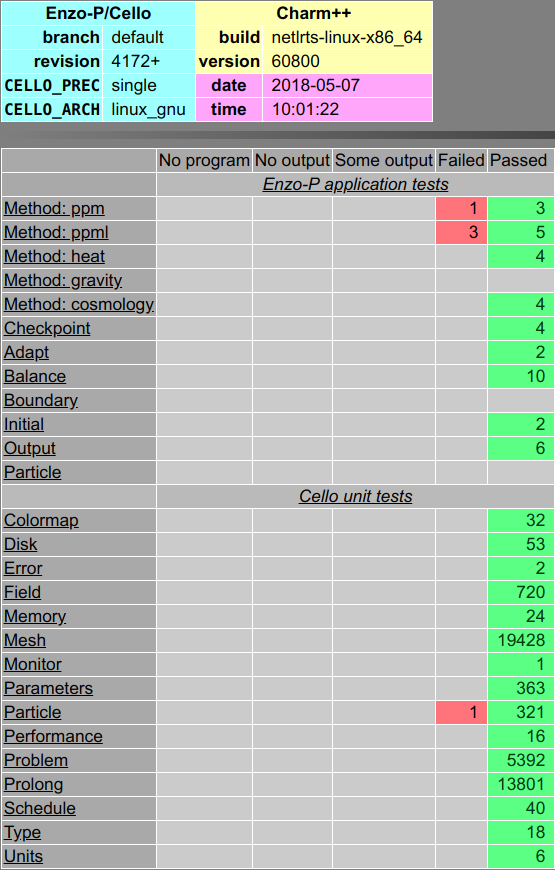
\includegraphics[width=1.75in]{Images/test-1.png}
\end{minipage} \ 
\begin{minipage}{2.25in}
\begin{itemize}
\item Summary of all tests
\item Columns:
\footnotesize
\begin{enumerate}
\item didn't compile
\item didn't start
\item didn't finish
\item tests failed
\item tests passed
\end{enumerate}
\small
\item A few failed tests are expected
\item Sections link to details
\end{itemize}
\end{minipage}
\end{frame}

%----------------------------------------------------------------------

\begin{frame}[fragile] 
\secframetitle{\ssTesting}
\framesubtitle{Enzo-P/Cello Test Results: adaptive mesh refinement}
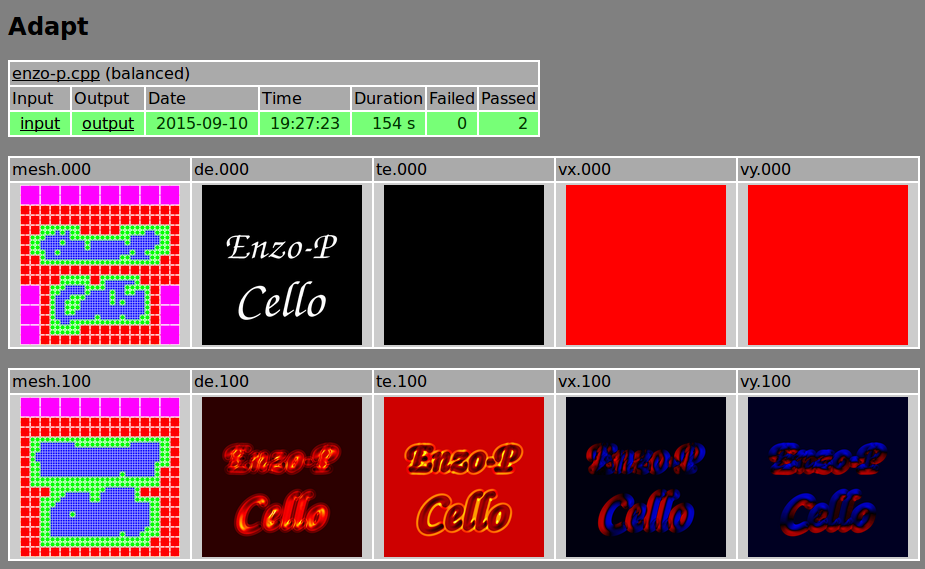
\includegraphics[width=4.0in]{Images/cello-test-2.png}
\end{frame}


\begin{frame}[fragile] 
\secframetitle{\ssTesting}
\framesubtitle{Enzo-P/Cello Test Results: dynamic load balancing}
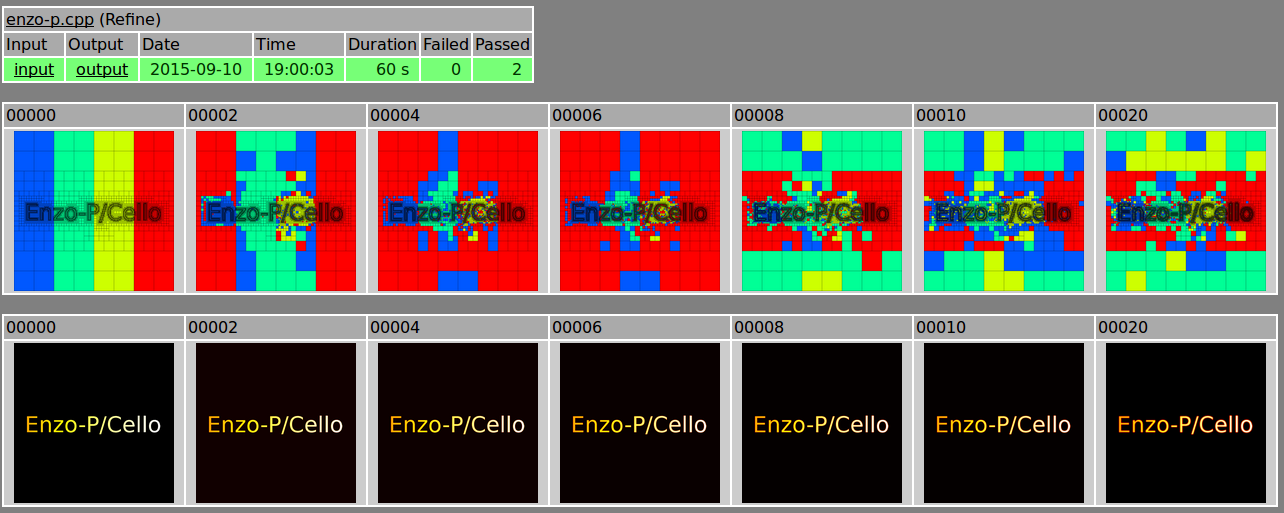
\includegraphics[width=4.0in]{Images/cello-test-3.png}
\end{frame}

 % How is testing done?
%======================================================================
\NEWSEC
%======================================================================

\subsection{\ssBugs}

\begin{frame}[fragile,label=ss-bugs] 
\secframetitle{\ssBugs}
\begin{itemize}
\item \greentext{\url{http://cello-project.org} / \framebox{Bug tracking}}
\end{itemize}
\rowcolors[]{1}{blue!5}{blue!10}
\begin{center}
\vspace{-0.1in}
\begin{minipage}{4.5in}
\footnotesize
\begin{tabular}{rll}
% (As of 2015-09-03)
% 2	2013-06-18 	Excessive syncronization during mesh adaptation 
% 3	2013-06-18 	Multiple refresh steps are performed 
% 4	2013-06-18 	ProlongLinear requires ghost depth of four 
% 12	2013-09-10 	Parallel runs may crash in inteuler with numerical errors 
% 13	2014-08-19 	I/O is incorrect for ip stride != 1 
% 19	2015-03-26 	method_ppm-1 and method_ppm-8 produce slightly different results
% 21	2014-03-17 	Small errors near corners of just-refined blocks 
% 31	2014-01-22 	Refresh errors in larger-scale parallel runs 
% 34	2014-02-21 	Several components seem to have memory leaks 
% 36	2014-03-17 	Adapt crashes (surprise) in sdsc-demo.in 
% 40	2014-04-29 	adapt-L5 problem fails sometimes 
% 45	2014-05-11 	Performance output for components seems incorrect 
% 46	2015-05-06 	Adapt seems to not be coarsening some blocks that should coarsen 
% 51	2014-06-27 	Parameter file syntax error messages display incorrect line number 
% 56	2014-08-21 	Restart fails when number of processors is changed 
% 57	2014-09-25 	stale Charm++ array messages in double mach problem cycle 846 
% 59	2014-11-20 	Occasional segmentation faults in file output from dereferencing null file_ pointer 
% 60	2015-07-06 	Load balancing unit tests occasionally hang 
% 68	2015-03-10 	Gravity solver still diverges sometimes 
% 72	2015-05-08 	RefineSlope does not work correctly sometimes 
% 73	2015-06-12 	New implementation of Refresh sometimes hangs sometimes crashes 
% 74	2015-06-16 	Enzo-P crashes in parse.l with Charm version 6.6.1 with P > 1 
% 75	2015-06-18 	method_heat-8 regression test failed 
% 76	2015-07-07 	Refresh add_fields() does not work as expected 
% 78	2015-07-15 	Mg0 solver has grid-effects 
% 79  	2015-07-27      Synchronization in Refresh is incorrect for Mg0
\uncover<1->{ID} & Date & \centerline{\uncover<1->{Summary}} \\
\hline
{\erow{151}} &	2018-05-03 &\erow{Single root block Cosmo crashes in refinement} \\
{\orow{150}} &	2018-04-26 &\orow{Memory leak in Cosmology problems} \\
{\erow{148}} &	2018-04-17 &\erow{load balancing fails when Index bit ordering is changed} \\
{\orow{147}} &	2018-04-17 &\orow{Errors with netlrs smp charm++} \\
{\erow{146}} &	2018-04-02 &\erow{Restart fails for Cosmo\_OsNa problem on SDSC Comet} \\
{\orow{138}} &	2018-02-07 &\orow{Image output fails with ``image\_ already created''} \\
{\erow{126}} &	2017-08-31 &\erow{data output of particles generates corrupt HDF5 files} \\
{\orow{118}} &	2017-07-12 &\orow{HDF5 output does not scale on Blue Waters} \\
{\erow{111}} & 	2017-06-08 &\erow{Adapt fails if octree array axis is not power of 2}
\end{tabular}
\end{minipage}
\end{center}
\end{frame}

 % What are some of the known bugs?
%======================================================================
\NEWSEC
%======================================================================

\subsection{\ssProjectSummary}

%----------------------------------------------------------------------

\begin{frame}[fragile,label=ss-project-summary] 
\secframetitle{\ssProjectSummary}
\begin{itemize}
\item The Enzo-P / Cello project is comprised of multiple components
\item Project page: \url{http://cello-project.org}
\item Source code
\begin{itemize}
\item  \code{http://bitbucket.org/cello-project}
\end{itemize}
\item Documentation
\begin{itemize}
\item doxygen auto-generated:  \code{cello-src/src-html}
\item restructured-text: \code{cello-doc/source}
\end{itemize}
\item Regression testing
\begin{itemize}
\item  \code{cello-src/test}
\item easy to run: \code{make test}
\item results easy to view: \code{cello-src/test/index.php}
\end{itemize}
\item Bug tracking and debugging
\begin{itemize}
\item Bugzilla: \url{http://cello-project.org/bug}
\item Debugging scripts: \code{cello-bug}
\end{itemize}
\end{itemize}
\vfill
\centerline{$\qed$}
\end{frame}

 
%%======================================================================
\NEWSEC
%======================================================================

\subsection{\ssCommunicate}

\begin{frame}[fragile,label=ss-communicate] 
\secframetitle{\ssCommunicate}
\end{frame}

 % How do Enzo-P developers communicate?
